%
% $Id: ch01_overview
%
%   *******************************************************************
%   * SEE THE MAIN FILE "AllegThesis.tex" FOR MORE INFORMATION.       *
%   *******************************************************************

\chapter{Introduction}\label{ch:intro} % we can refer to chapter by the label

The Spotify API allows public access to an ever-growing list of end points
for every song in their 40 million and growing music catalog. Despite this vast
wealth of information, Spotify users are not allowed to select tracks based on this
data. This chapter lists the driving motivations for this project, analyzes other
ventures into Spotify API data, and outlines the goals and vision for this
application.
\section{Motivation} \label{sec:motivation}

The personal motivations for this project stemmed from a series of criteria that
I wanted my thesis to fulfil, before choosing a specific project to pursue. The
requirements included:
\begin{itemize}
  \item Inclusion of music - As an active musician at Allegheny College, as well
  as a music theory minor, it almost went without saying that I wanted to include
  my biggest passion in a senior research project.

  \item Practicality - I sought to create a project that, at the very least, could
  likely have continued real-world utilization by myself (and hopefully others)
  after the conclusion of my academic career.

  \item Opportunity to learn - Being not well-versed in working with existing APIs,
  as well as the area of both front-end and back-end web development, I saw this
  assignment as an opportunity to explore areas I was not able to through college
  courses
\end{itemize}

Apart from these self-defined criteria, after settling on the specific topic of playlist
creation, the Spotify API itself served as motivation. My simultaneous amazement of
the power that Spotify holds, as well as frustration for the lack of use and support
of the breadth of data generated, was enough to begin creating a tool to remedy
this shortfall in music discovery.

Spotify currently controls 36\% of the global music streaming market \cite{Midia:18}. With a
catalog of well over 40 million songs, there is an abundance of music to fit
any listeners' taste. Despite this, Spotify has no easy way to use the information
Spotify collects to sort and choose songs, other than a selection of premade playlists
for diferent genres and keywords. Artist pages include tabs categorizing related artists,
but there is no way to quickly generate a list of songs that
takes advantage of the track information Spotify possesses. The Spotify
API can allow for this and much more, but curated music discovery is limited to one weekly
playlist, called "Discover Weekly", consisting of 30 songs tailor made for each
Spotify user. As accurate as this playlist is, it merely scratches the surface of
what the data that Spotify possesses can achieve. With so much more data on every
song in Spotify's library already available, the motivation for this project is
simple: allowing Spotify customers to find new music at any time, with any selected
specifications, puts the power of discovery in their hands. Finding new songs is
always enjoyable, and this project can create that feeling at a user's disposal.


\section{Current State of the Art}\label{sec:stateofart}

In 2014, Spotify acquired the music intelligence company "The Echo Nest" \cite{echo:14}.
The company collects hundreds of data points on songs, such as values for the key,
tempo, song duration, time signature, and other features. They have also created
formulas to calculate more abstract features, including energy and "danceability".
These values are composites of simpler points; energy is based on overall loudness
of a song, as well as segment duration, which refers to loops and repeated sections
of songs. The danceability formula has not been released, but is a combination of
beat strength, tempo and tempo stability, and other undisclosed factors. Spotify
gaining control of the company gave them access to this database, and a year later
the Discover Weekly playlist was released \cite{Constine:15}.

The Discover Weekly playlist is so successful because of the way it is tailored to
Spotify customers. The first deciding portion is pulled from the user's
"taste profile", aggregated from songs a user listens to, or saves to their library.
The profile is grouped into clusters, such as this example for reporter Nikhil Sonnad
\cite{Pasick:15}:

\begin{center}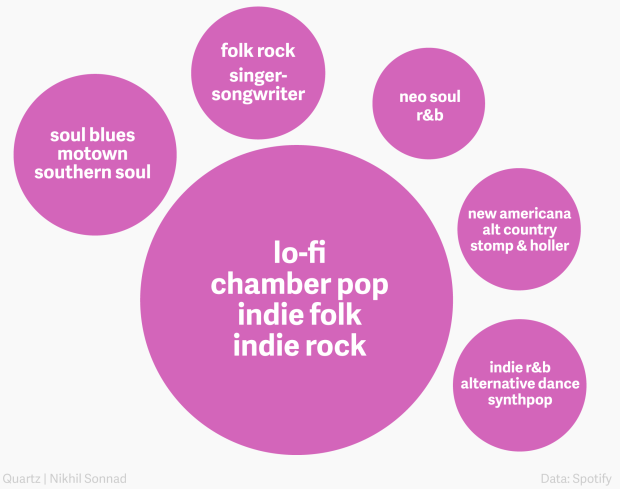
\includegraphics[height=6cm]{images/cluster-genres.png}

\end{center} Fine-grained genres, such as "chamber pop", or "stomp \& holler", are taken from
methods from The Echo Nest, and are used as a first level of personalization. The cluster-based
approach serves to eliminate many songs that users will not be interested in, but also allow
multiple wide-spanning genres that may have no relation with each other.

The other prong of the Discover Weekly method is collaborative filtering \cite{Ciocca:17}. For
Spotify, this technique works by comparing users who have played many of the same tracks in
the same genre. Spotify creates a giant matrix to compare the songs, with each row corresponding
to one of the 140 million users, and a column for each song in their catalog \cite{Spotify:15}.
\begin{center}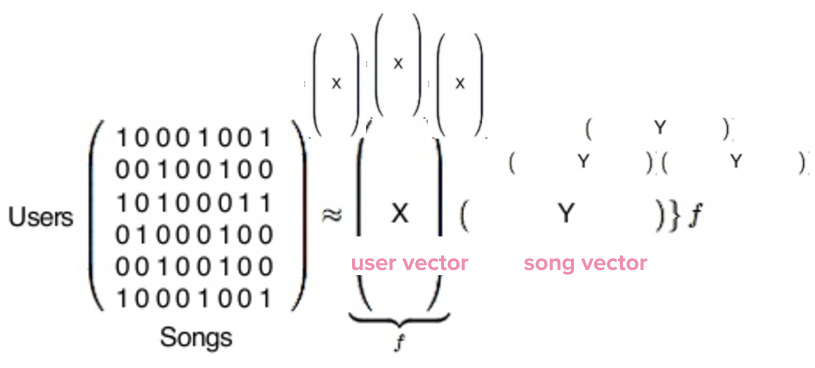
\includegraphics[height=6cm]{images/matrix.png}

\end{center} The user vectors, represented by columns in the matrix, are compared
with each other to find their closest matches, determined by similar patterns of
interactions with the same tracks. Songs which appear
in user's A's vector, but not in user B's, are recommended to user B. The end
result is a playlist of music which feels handpicked by a close friend, but is
actually the result of a cleverly crafted algorithm. Currently, the Discover Weekly
playlist is the gold standard for personalized music discovery. Millions of users
receive a list of songs they are likely to enjoy, every week without fail.

\section{Goals of the Project}\label{sec:goals}

As this project is an academic thesis, and not just a simple weekend hobby, my
overarching objective is to demonstrate what I have been able to learn at
Allegheny College, as a capstone to end my academics. More specifically to this
tool, I wish to prove my ability to meld my passion of music, with my major of
computer science. In this process, I wish to research utilization of established,
robust APIs, to create an application that shows principles which can be brought
with me into the professional industry. Upon beginning this thesis project, I have
just elementary experience on working with APIs, and even less knowledge of web
development. With these shortcomings in mind, my primary goal in completing this
thesis is to develop a working ability in these areas as such:

\begin{itemize}
  \item Spotify API - be able to call information from Spotify's database, in a
  way which allows music listeners greater control over tracks they listen to.

  \item Web Development - Explore front-end and back-end web development strategies,
  as well as the use of framework and bootstrap tools, to package my tool in a more
  logical and accessible way for public use.
\end{itemize}

Concerning goals within the scope of the tool, the objective of this project is
to create a web-based application which allows music fans of all levels to create
fine-tuned playlists, based on any amount of available criteria. As previously
discussed, the Discover Weekly playlist is the premier tool for finding song
tracks unrecognized to the user. However, the tool has its own set of drawbacks.
Since both methods use Spotify customer behavior to create parameters, non-subscribers
will not be able to use the feature at all, and less active or new subscribers will
not have a baseline for the technique to begin from. In addition, the playlist
only refreshes once a week, giving thirty new tracks. There is no way to manually
reset your playlist, or get more new songs. The project I outline would be web-based,
using the data that Spotify already possesses. Using the Spotify
API, I will create a custom playlist which could be played in the page, or saved to a user's
profile. The input for the tool would be any song in the Spotify catalog, or alternatively
genres or certain keywords. Keywords would be words that appear in popular playlist titles,
and tracks would be selected from them. In addition to this user input, there will also be
options to adjust ranges of features that are inherent to every song, such as overall song
popularity, tempo, energy, amount of vocals present, and other characteristics. These metrics
allow fans to fine tune the resulting playlist, ensuring they will be able to find enjoyable
tracks, making finding new songs an easy task for any music fan.

Considering this project heavily involves something I am passionate about, I foresee
myself adding features, and increasing the robustness of this application, for years
to come down the road. The Spotify API is constantly adding features and increasing
available information, so the final state of this project is apt to change after
the conclusion of the academic year. Because of this possibility, it is important
that I do not lose track of the scope and time available. Especially for areas I
have less experience with, success may be defined as having a working "proof of
concept", and a fully functional web-app may have to be completed at a later time.
My final goal is to enjoy the process of creating a working product, which should
be aided by the subject matter.

\section{Thesis Statement}\label{sec:statement}

This thesis project is an application stemming heavily from research into the
Spotify API, as well as various strategies utilized for hosting the playlist
creator and editor methods in a web-app. The resulting product will be designed
to allow any user to edit and create Spotify playlists, taking advantage of the
end points of tracks in the Spotify catalog. The target audience is music fans
of any level of theory knowledge, so making the application both usable and accessible
for anyone is a major design concern. Research into the Spotify API will directly
impact the design and output of the project.

\section{Thesis Outline}\label{sec:outline}

Chapter \ref{ch:music} outlines the idea of Music Information Retrieval, as well as how the
field has been used in existing Spotify projects. Chapter \ref{ch:method} gives a framework of
how the Spotify API is structured, as well as outlines of Spotipy and Flask. Chapter
\ref{ch:implem} outlines the initial design of the project, including specific code
examples to better explain the product. Chapter \ref{ch:conclusion} lists future
improvements that are desired, as well as new conceptual features.
